\documentclass[tikz,border=6pt,12pt]{standalone}
\usepackage{tikz}
\usetikzlibrary{shapes.symbols,matrix,positioning,automata,fit,arrows.meta,calc,quotes, bending}

\begin{document}
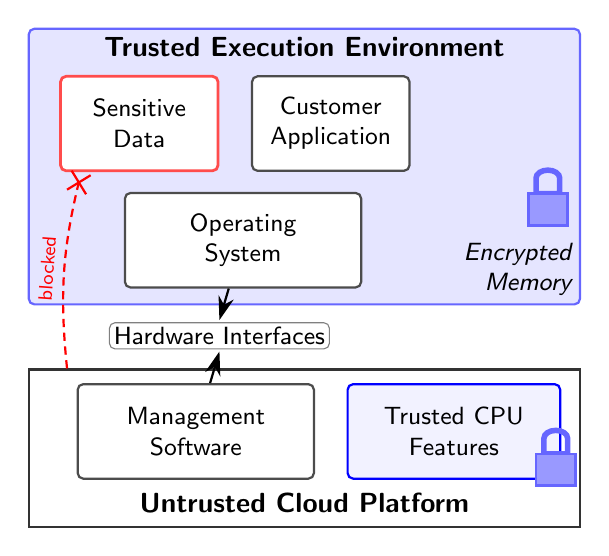
\begin{tikzpicture}[
    font=\sffamily\small,
    teeBlue/.style={fill=blue!10,draw=blue!60,thick,rounded corners=2pt},
    box/.style    ={draw=black!70,rounded corners=2pt,thick,align=center},
    lbl/.style    ={font=\sffamily\bfseries},
    it/.style    ={font=\sffamily\itshape},
    arrow/.style  ={->,>={Stealth[length=3mm,width=2mm]},thick},
]

\tikzset{
  pics/padlock/.style={
    code={
      \draw[line width=2pt,draw=blue!60]
        (-0.15,0) arc (180:0:0.15 and 0.1) -- ++(0,-0.2) -- ++(-0.3,0) -- cycle;
      \draw[line width=1pt,fill=blue!40,draw=blue!60]
        (-0.25,-0.2) rectangle (0.25,-0.6);
    }
  }
}

% ---------- Parameters (all unit-less, treated as cm later) ----------
\def\W{7.0}    % total width
\def\Htop{3.5}  % TEE height
\def\Hbot{2.0}  % platform height
\def\gap{0.4}   % vertical gap
\def\pad{0.4}   % inner padding

\def\leftW{4.7} % left column width inside TEE
\def\rowH{1.2}  % row height for left-column boxes

% Derived widths (unit-less numbers)
\pgfmathsetmacro{\cpuW}{\W - 7.2 - 2*\pad - 0.5}

% ---------- Top: VM-Level TEE ----------
\node[teeBlue, minimum width=\W cm, minimum height=\Htop cm, anchor=north west] (TEE) at (0,0) {};
\node[anchor=north, lbl] at ([xshift=0pt,yshift=-0pt]TEE.north) {Trusted Execution Environment};


% Left column (three stacked boxes)
\node[box, minimum width=2 cm, minimum height=\rowH cm, draw=red!70,line width=1pt, anchor=north west, fill=white]
  (SD) at ([xshift=\pad cm,yshift=-0.6cm]TEE.north west) {Sensitive\\Data};
\node[box, minimum width=2 cm, minimum height=\rowH cm,  fill=white, anchor=west]
(APP) at ([xshift=\pad cm]SD.east) {Customer\\Application};
\node[box, minimum width=3 cm, minimum height=\rowH cm, anchor=north, fill=white]
  (OS) at ([xshift=.3cm, yshift=-0.25cm]SD.south east) {Operating\\System};

% Right region: Encrypted Memory
\node[anchor=south east, align=right,font=\itshape\small\sffamily]
      (ENC) at (TEE.south east)
      {Encrypted\\Memory};

% ---------- Bottom: Untrusted Cloud Platform ----------
\node[draw=black!80,thick,minimum width=\W cm, minimum height=\Hbot cm, anchor=north west]
      (PLAT) at ([yshift= -.8 cm]TEE.south west) {};

\node[anchor=south, lbl] at ([yshift=2pt]PLAT.south) {Untrusted Cloud Platform};

% VMM (left)
\node[box, fill=white, minimum width=3cm, minimum height=\rowH cm, anchor=north]
      (VMM) at ([xshift=-.6 cm,yshift=-1.2 cm]OS.south) {Management\\Software};

% Trusted CPU Features  + padlock
\node[box, fill=blue!5, minimum width=2.7 cm, minimum height=\rowH cm,
      anchor=west, draw=blue, thick]
      (CPU) at ([xshift=\pad cm,yshift=0 cm]VMM.east) {Trusted CPU\\Features};



% ---------- Hardware Interfaces (double arrow & label) ----------
\path let \p1 = (OS.south), \p2 = (VMM.north) 
	in node (mid) at ($(\p1)!.5!(\p2)$) {};

% \draw[arrow,dotted] (SP) -- (APP) node[midway,sloped,above]{provides};
% \draw [-{Latex[length=1.5mm]},dotted] (leaf_1) to [bend left=30]  node [above, sloped]  (TextNode2) {$d_1$} (biomass_pool);
\draw[arrow,>={Rays[length=10pt]},color=red, densely dashed]
	([xshift=.5cm]PLAT.north west)  to [bend left=10] 
	node[above,sloped,align=left,font=\scriptsize\sffamily](TEXT){blocked}
	(SD.220)
;

\draw[arrow] (OS) -- ($(mid)+(0,0.20)$);
\draw[arrow] (VMM) -- ($(mid)+(0,-0.20)$);
\node[fill=white, inner sep=1.6pt, draw=black!50, rounded corners=2pt] at (mid) {Hardware Interfaces};

% Padlocks
\pic at ([xshift=-12pt,yshift=20pt]ENC.north east) {padlock};
\pic at ([xshift=-2 pt,yshift=15pt]CPU.south east) {padlock};

\end{tikzpicture}
\end{document}
